\documentclass[10pt,pdf,hyperref={unicode}]{beamer}

\mode<presentation>
{
\usetheme{boxes}
\beamertemplatenavigationsymbolsempty

\setbeamertemplate{footline}[page number]
\setbeamersize{text margin left=1em, text margin right=0.5em}
}

\usepackage[utf8]{inputenc}
\usepackage[english, russian]{babel}
\usepackage[normalem]{ulem}
\usepackage{bm}
\usepackage{multirow}
\usepackage{ragged2e}
\usepackage{indentfirst}
\usepackage{multicol}
\usepackage{subfig}
\usepackage{amsmath,amssymb}
\usepackage{dsfont}
\usepackage{enumerate}
\usepackage{mathtools}
\usepackage{comment}
\usepackage{tabularx, tabulary, multicol}
\usepackage[all]{xy}

\newcommand{\bz}{\mathbf{z}}
\newcommand{\bx}{\mathbf{x}}
\newcommand{\by}{\mathbf{y}}
\newcommand{\bv}{\mathbf{v}}
\newcommand{\bw}{\mathbf{w}}
\newcommand{\ba}{\mathbf{a}}
\newcommand{\bb}{\mathbf{b}}
\newcommand{\bff}{\mathbf{f}}
\newcommand{\bh}{\mathbf{h}}
\newcommand{\bl}{\mathbf{l}}
\newcommand{\bp}{\mathbf{p}}
\newcommand{\bq}{\mathbf{q}}
\newcommand{\bs}{\mathbf{s}}
\newcommand{\bt}{\mathbf{t}}
\newcommand{\bu}{\mathbf{u}}
\newcommand{\bT}{\mathbf{T}}
\newcommand{\bX}{\mathbf{X}}
\newcommand{\bZ}{\mathbf{Z}}
\newcommand{\bS}{\mathbf{S}}
\newcommand{\bH}{\mathbf{H}}
\newcommand{\bW}{\mathbf{W}}
\newcommand{\bY}{\mathbf{Y}}
\newcommand{\bU}{\mathbf{U}}
\newcommand{\bQ}{\mathbf{Q}}
\newcommand{\bP}{\mathbf{P}}
\newcommand{\bA}{\mathbf{A}}
\newcommand{\bB}{\mathbf{B}}
\newcommand{\bC}{\mathbf{C}}
\newcommand{\bE}{\mathbf{E}}
\newcommand{\bF}{\mathbf{F}}
\newcommand{\bsigma}{\boldsymbol{\sigma}}
\newcommand{\bomega}{\boldsymbol{\omega}}
\newcommand{\btheta}{\boldsymbol{\theta}}
\newcommand{\bgamma}{\boldsymbol{\gamma}}
\newcommand{\bdelta}{\boldsymbol{\delta}}
\newcommand{\bPsi}{\boldsymbol{\Psi}}
\newcommand{\bpsi}{\boldsymbol{\psi}}
\newcommand{\bxi}{\boldsymbol{\xi}}
\newcommand{\bmu}{\boldsymbol{\mu}}
\newcommand{\bchi}{\boldsymbol{\chi}}
\newcommand{\bzeta}{\boldsymbol{\zeta}}
\newcommand{\blambda}{\boldsymbol{\lambda}}
\newcommand{\beps}{\boldsymbol{\varepsilon}}
\newcommand{\bZeta}{\boldsymbol{Z}}
% mathcal
\newcommand{\cX}{\mathcal{X}}
\newcommand{\cY}{\mathcal{Y}}
\newcommand{\cW}{\mathcal{W}}

\newcommand{\dH}{\mathds{H}}
\newcommand{\dR}{\mathds{R}}
% transpose
\newcommand{\T}{^{\mathsf{T}}}

% command to strike out text
\newcommand{\stkout}[1]{\ifmmode\text{\sout{\ensuremath{#1}}}\else\sout{#1}\fi}

% limited alertblock
\newenvironment<>{varblock}[2][.9\textwidth]{%
	\setlength{\textwidth}{#1}
	\begin{actionenv}#3%
		\def\insertblocktitle{#2}%
		\par%
		\usebeamertemplate{block begin}}
	{\par%
		\usebeamertemplate{block end}%
	\end{actionenv}}

\renewcommand{\epsilon}{\ensuremath{\varepsilon}}
\renewcommand{\phi}{\ensuremath{\varphi}}
\renewcommand{\kappa}{\ensuremath{\varkappa}}
\renewcommand{\le}{\ensuremath{\leqslant}}
\renewcommand{\leq}{\ensuremath{\leqslant}}
\renewcommand{\ge}{\ensuremath{\geqslant}}
\renewcommand{\geq}{\ensuremath{\geqslant}}
\renewcommand{\emptyset}{\varnothing}

\usepackage{tikz}
\usetikzlibrary{positioning,arrows}

\tikzstyle{name} = [parameters]
\definecolor{name}{rgb}{0.5,0.5,0.5}

\usepackage{caption}
\captionsetup{skip=0pt,belowskip=0pt}

\newtheorem{rustheorem}{Теорема}
\newtheorem{russtatement}{Утверждение}
\newtheorem{rusdefinition}{Определение}

% colors
\definecolor{darkgreen}{rgb}{0.0, 0.2, 0.13}
\definecolor{darkcyan}{rgb}{0.0, 0.55, 0.55}

\AtBeginEnvironment{figure}{\setcounter{subfigure}{0}}

\captionsetup[subfloat]{labelformat=empty}
\addto\captionsrussian{\renewcommand{\figurename}{}}
\graphicspath{{../figures/}}

%----------------------------------------------------------------------------------------------------------

\title[Заголовок]{Генеративный причинно-следственный подход к анализу данных нейроинтерфейсов}
\author{Владимиров Э.А.}

\institute[]{Московский физико-технический институт}
\date{\footnotesize
	\par\smallskip\emph{Научный руководитель:} д.~ф.-м.~н. В.\,В.~Стрижов
	\par\bigskip\small 2025}

%---------------------------------------------------------------------------------------------------------
\begin{document}

\begin{frame}
\titlepage
\end{frame}

%----------------------------------------------------------------------------------------------------------
\begin{frame}{Причинно-следственный анализ}
	\begin{alertblock}{Проблема обнаружения связи}
		\begin{itemize}
			\item[-] Традиционные методы (корреляция, линейная регрессия) неадекватны для сложных нелинейных связей.
			\item[-] Данные имеют высокую размерность, что усложняет поиск причинно-следственных связей.
			\item[-] Зависимости между переменными могут изменяться во времени.
		\end{itemize}
	\end{alertblock}
	
	\begin{alertblock}{Требуется}
		Построить устойчивую и интерпретируемую форму вероятностного анализа причинного влияния $\bX \rightarrow \bY$.
	\end{alertblock}

	\begin{alertblock}{Решение}
		Предлагается следующий подход ПАНКВИ ~--- Причинный Анализ на основе Независимых Компонент и Взаимной Информации: 
		
		Метод независимых компонент $\longrightarrow$ восстановление фазового пространства $\longrightarrow$ вычисление взаимной информации.
	\end{alertblock}
\end{frame}

%---------------------------------------------------------------------------------------------------------
\begin{frame}{Различные подходы к поиску связей}
%	\begin{figure}
%		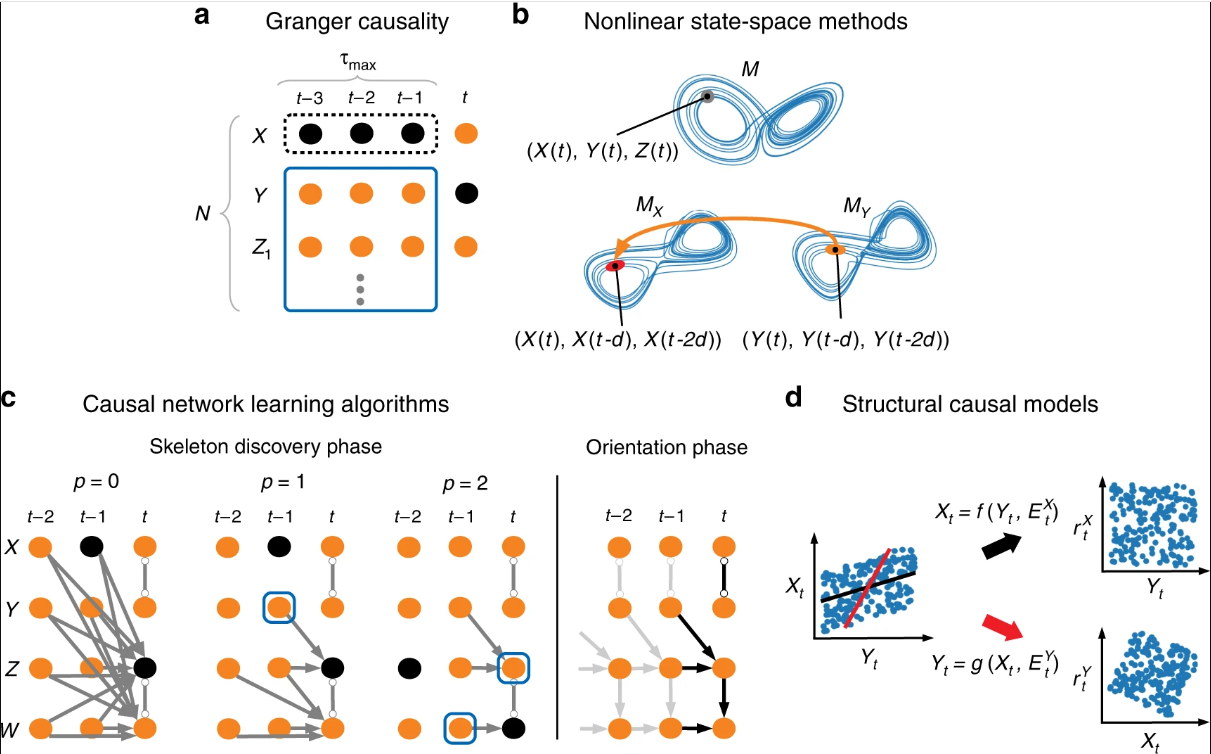
\includegraphics[width=0.6\linewidth]{ci-approaches}
%		\caption{Существующие подходы}
%	\end{figure}

	\begin{figure}
		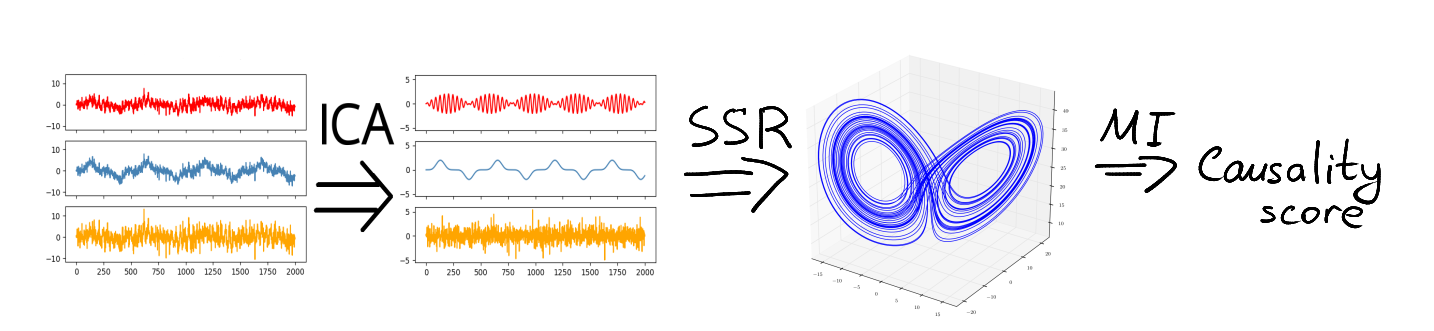
\includegraphics[width=\linewidth]{ica-ssr-mi}
		\caption{Предлагаемый подход ПАНКВИ}
	\end{figure}
\end{frame}

%--------------------------------------------------------------------------------------------------------

\begin{frame}{Постановка задачи обнаружения связи}
	Даны \( \mathbf{X}(t) = \{X_1(t), X_2(t), \ldots, X_{n_x}(t)\} \) и \( \mathbf{Y}(t) = \{Y_1(t), Y_2(t), \ldots, Y_{n_y}(t)\} \) — набор временных рядов, наблюдаемых в моменты времени \( t = 1, \ldots, T \).
	
	Необходимо определить направленные причинные связи:
		$$ X_i(t-\tau) \to Y_j(t) \text{ и } Y_j(t-\tau) \to X_i(t) $$
		
	для \( i = 1, \ldots, n_x \), \( j = 1, \ldots, n_y \), и лагов \( \tau \geq 0 \),
	
	Предполагаем, что многомерные временные ряды \( \mathbf{X}(t) \) и \( \mathbf{Y}(t) \) генерируются следующим образом:
	\[
	X_i(t) = f_i(\text{Pa}_{X_i}(t), \varepsilon_{X_i}(t)),
	\]
	\[
	Y_j(t) = g_j(\text{Pa}_{Y_j}(t), \varepsilon_{Y_j}(t)),
	\]
	где:
	\begin{enumerate}
		\item[-] $ \text{Pa}_{X_i}(t), \; \text{Pa}_{Y_j}(t)$ — множество родителей  переменных $ X_i(t) \text{ и } Y_j(t) $ из \( \mathbf{Y} \) и \( \mathbf{X} \) соответственно,
		\item[-] \( f_i \) и \( g_j \) — детерминированные функции, описывающие зависимость,
		\item[-] \( \varepsilon_{X_i}(t) \) и \( \varepsilon_{Y_j}(t) \) — шумовые компоненты.
	\end{enumerate}
\end{frame}

%---------------------------------------------------------------------------------------------------------
\begin{frame}{Метод независимых компонент}
	Предположим, что $\mathbf{X}(t)$ образуется из нескольких скрытых источников $\mathbf{S}(t)\in \mathbb{R}^{d_S}$:
	\[
		\mathbf{X}(t) \;=\; A\,\mathbf{S}(t) 
	\]
	
	Каждая компонента $S_k(t)$ предполагается статистически независимой от других:
		\[
		p(\mathbf{S}) = p(S_1, S_2, \ldots, S_{d_S}) = \prod_{k=1}^{d_S} p\bigl(S_k\bigr).
		\]
	
	\textbf{Задача оптимизации:}
		Минимизировать взаимную информацию между компонентами $\widehat{S}_k(t)$.
		\[
		\mathrm{MI}\bigl(\widehat{\mathbf{S}}(t)\bigr) 
		\;\approx\; 
		\sum_{k=1}^{d_S} H\bigl(S_k\bigr) - H\Bigl(\sum_k S_k\Bigr),
		\]
		найдя обратный линейный оператор $\widehat{A}^{-1}$
		\[
		\widehat{\mathbf{S}}(t) 
		\;=\; 
		\widehat{A}^{-1}\,\mathbf{X}(t).
		\]

\end{frame}
%----------------------------------------------------------------------------------------------------------
\begin{frame}{Сходящийся перекрестный анализ}
	\textbf{Теневое вложение:}
	\[
	M_{X,t}
	= 
	\bigl(
	X_t,\,
	X_{t-\tau},\,
	\dots,\,
	X_{t-(E-1)\tau}
	\bigr)
	\;\in\;\mathbb{R}^E,
	\]
	где $E$ --- размерность вложения, $\tau$ --- временной лаг. 
	%Аналогично задаётся $M_{Y,t} = \bigl(Y_t,\,Y_{t-\tau},\,\dots\bigr).$
	
	\vspace{1em}
	\textbf{Реконструкция:}
	\[
	\widehat{Y}_t | M_{X, t}
	=
	\sum_{i=1}^{k}
	w_i\,
	Y_{n_i},
	\]
	здесь $n_i$ --- индексы ближайших соседей точки $M_{X,t}$ в пространстве $M_X$, а $w_i$ --- веса, зависящие от расстояния до $M_{X,t}$.
	
	\vspace{1em}
	\textbf{Критерий причинности:}
	\[
	\rho_{X\to Y}
	=
	\mathrm{corr}\!\Bigl( Y_t, \widehat{Y}_t | M_{X, t} \Bigr).
	\]
	Если при увеличении размера ``библиотеки'' (множества рассматриваемых соседей) $\rho_{X \to Y}$ \emph{сходится монотонно}, считается, что $\mathbf{X}(t)$ влияет на $\mathbf{Y}(t)$.
\end{frame}

%----------------------------------------------------------------------------------------------------------
\begin{frame}{Вероятностный перекрёстный анализ}
	Рассматриваем $p\bigl(Y_t \mid M_{X,t}\bigr)$ и $p(Y_t)$ вместо точечных значений.
	
	\vspace{1em}
	\textbf{Взаимная информация как оценка причинности}
	
	Вместо корреляции, в качестве оценки причинно-следственной связи возьмём взаимную информацию:
		
	\[
	Prob_{CCM}(X, Y) = MI(M_X, Y) = 
	\mathbb{E}_{X}
	D_{\mathrm{KL}}\!\Bigl[
	p\bigl(Y \mid M_X \bigr)
	\;\big\|\;
	p\bigl(Y\bigr)
	\Bigr],
	\]
	
	\vspace{1em}
	\textbf{Направленная связь и относительная взаимная информация}  
	
	Поскольку взаимная информация ~--- симметричная функция, то для оценки однонаправленных связей необходимо воспользоваться условной взаимной информацией:
	
	\[MI(X, Y | Y_{hist}) = \mathbb{E}_{X, Y_{hist}} D_{\mathrm{KL}} \Bigl[ p(Y | M_X, Y_{hist} ) \| p(Y | Y_{hist}) \Bigr] \]

\end{frame}

%----------------------------------------------------------------------------------------------------------
\begin{frame}{Предлагаемый метод ПАНКВИ}
	\begin{enumerate}
		\item \textbf{Независимый анализ компонент}\\
		Для исходных ЭЭГ-данных $\mathbf{X}(t)\in\mathbb{R}^{d_X}$ получаем независимые компоненты:
		\[
		\widehat{\mathbf{S}}(t) 
		= 
		\widehat{A}^{-1}\,\mathbf{X}(t).
		\]
		
		\vspace{0.5em}
		\item \textbf{Восстановление фазового пространства}\\
		Для каждого времени $t$ формируем вектор:
		\[
		M_{X,t} = 
		\bigl(\widehat{\mathbf{S}}(t),\,\widehat{\mathbf{S}}(t-\tau),\dots,\widehat{\mathbf{S}}(t-(E-1)\tau)\bigr),
		\]
		
		\vspace{0.5em}
		\item \textbf{Оценка причинно-следственных связей}\\
		В полученном пространстве $(M_{X,t},\,M_{Y,t})$ определяем для каждого $l \in \{ 1, \ldots, d_y\}$ оценку влияния $\mathbf{X} \to Y_l(t)$, вычисляя:
		\[
		\mathrm{Prob_{CCM}}\bigl(M_{X,t}, Y_l(t)\bigr).
		\]
		Аналогично, для каждого $m \in \{ 1, \ldots, d_x \}$ вычисляем $\mathrm{Prob_{CCM}}\bigl(M_{Y,t}, X_m(t)\bigr).$.
		
	\end{enumerate}
\end{frame}

%----------------------------------------------------------------------------------------------------------
\begin{frame}{Альтернативная постановка задачи обнаружения связи}
	Причинно-следственная связь ~--- вероятность диффеоморфизма.
	
	Основная проблема ~--- построение многообразий
	
	\vspace{0.5em}
	
	\textbf{Опр.} \textit{Причинно-следственный механизм} ``$X \rightarrow Y$'' это марковское ядро:
	$
	\kappa(y|x) : \mathcal{X} \to \mathbb{P}(\mathcal{Y})
	$
	
	\vspace{0.5em}
	\textbf{Опр.} Пусть $\mathcal{M}_{\mathcal{X}}, \; \mathcal{M}_{\mathcal{Y}}$ – статистические многообразия мер на $\mathcal{X}$ и $\mathcal{Y}$. Назовём \textit{отображением эффекта} $\mathbb{T}_{\kappa} : \mathcal{M}_{\mathcal{X}} \rightarrow \mathcal{M}_{\mathcal{Y}}$:
	
	$$
		\mathbb{T}_{\kappa}(P_X) = P_X \ast \kappa, \text{ то есть }
		\mathbb{T}_{\kappa}(P_X)(B) = \int_{x} \kappa(B|x) \, P_X(dx)
	$$
	
	Эффект $(P_X \rightarrow Q_X) = \text{Изменение}\left(\mathbb{T}_{\kappa} P_X \rightarrow \mathbb{T}_{\kappa} Q_X\right)$
	
	\vspace{0.5em}
	\textbf{Задача обнаружения причинно-следственной связи} ~--- построение $\mathbb{T}_{\kappa}$ или определение её свойств на основе данных.
	
	\vspace{0.5em}
	\textbf{Пример:} $do(X = x_0) \Leftrightarrow P_X = \delta_{x_0}$ \\
	Тогда,
	\[
	\mathbb{T}(\delta_{x_0}) = \kappa(\cdot | x_0) = \mathbb{P}(Y | do(X = x_0))
	\]
	
\end{frame}

%----------------------------------------------------------------------------------------------------------
\begin{frame}{Вычислительный эксперимент на данных ЭЭГ - ИИМ}	
	\begin{multicols}{2}
	
		\begin{varblock}[6cm]{Данные}
			У 25 участников были записаны показания ЭЭГ, ИИМ, МРТ во время игры в настольный теннис. С каждым участником было сыграно 4 сессии, длительность каждой из них составляет 7-10 минут.
		\end{varblock}
	
		\begin{figure}
			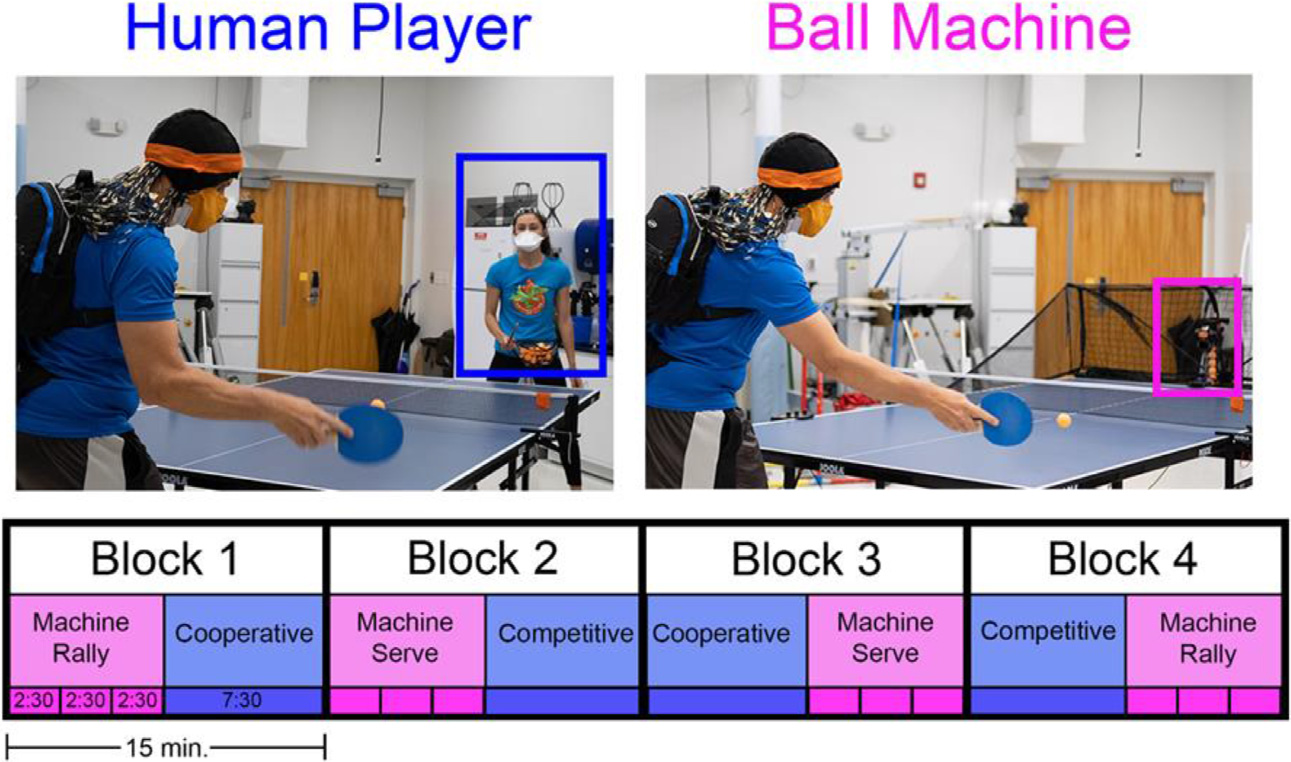
\includegraphics[width=\linewidth]{tennis-viz.png}
		\end{figure}

	\end{multicols}
\end{frame}

\begin{frame}{Выносится на защиту}
	\begin{enumerate}
		\item Проведено сравнение методов выявления причинно-следственных связей
		
		\item Предложен новый способ обнаружения связей, учитывающий высокую размерность данных и нелинейную связь компонент
		
		\item Представлена альтернативная постановка задачи обнаружения связи, которая будет развиваться в дальнейшем
		
		% \item Проведён вычислительный эксперимент на данных ЭЭГ - ИИМ, в котором метод доказал свою корректность
		
	\end{enumerate}
\end{frame}

\end{document} 
